%!TEX root = lec06_transactions.tex

%
% ----------------------------------------
%
\begin{frame}{Atomicity and Durability with logging}

There are two ways the DBMS can violate the atomicity principle:
\begin{itemize}[-,noitemsep,topsep=1pt]
\item When some write operation of a transaction that commits is not made persistent.
\item When some write operation by a transaction that aborts is made persistent.
\end{itemize}

\vskip0.5em

Because transactions take time to complete, and computers do crash, the DBMS keeps a log of the operations performed by a transaction.

\vskip0.5em

If the DBMS crashes during the execution of a transaction, the crash recovery system uses the log to ensure atomicity.

\end{frame}

%
% ----------------------------------------
%
\begin{frame}{Undo Logging}

\textbf{Idea}: save the values the database elements had before the transaction started in the log. If there is a problem, revert to them.

\vskip1em

\textbf{Rules}
\begin{enumerate}[(1)]
\item On a call to \WRITE{X}{v} by transaction $T_j$, write to the log the \textbf{old} value of database element \texttt{X}.
\item Only write \LOGCOMMIT{j} to the log \textbf{after} all new values are written (through a call to \OUTPUT{$\cdot$})
\end{enumerate}

\vskip1em

\begin{block}{Write Ahead Logging (WAL)}
Write all old values to the log before writing any new values to disk.
\end{block}
\end{frame}

\newsavebox{\undoLoggingExample}
\savebox{\undoLoggingExample}{%
\footnotesize
\begin{tabular}{r|l|r|r|r|r|r|l}
& & & \multicolumn{2}{|c|}{Memory} & \multicolumn{2}{|c|}{Disk} & \\
\cline{4-7}
\raisebox{0.75em}{Step} & \raisebox{0.75em}{Action} & \raisebox{0.75em}{\texttt{v}} & \texttt{A} & \texttt{B} & \texttt{A} & \texttt{B} & \raisebox{0.75em}{Log} \\
\hline
1 & &&&& 75 & 40 & \LOGSTART{1}\\
2 & \READ{A}{v} & 75 & 75 &  & 75 & 40 \\
3 & \ASSIGN{v}{v-20} & 55 & 75 &  & 75 & 40 \\
4 & \WRITE{A}{v} & 55 & 55 &  & 75 & 40 & \LOGUNDO{1}{A}{75}\\
5 & \READ{B}{v} & 40 & 55 & 40 & 75 & 40 \\
6 & \ASSIGN{v}{v+20} & 60 & 55 & 40 & 75 & 40 \\
7 & \WRITE{B}{v} & 60 & 55 & 60 & 75 & 40 & \LOGUNDO{1}{B}{40}\\
8 & \OUTPUT{A} & -- & 55 & 60 & 55 & 40  \\
9 & \OUTPUT{B} & -- & 55 & 60 & 55 & 60  \\
10 & \COMMIT & -- & 55 & 60 & 55 & 60 &  \LOGCOMMIT{1} \\
\end{tabular}
}

%
% ----------------------------------------
%
\begin{frame}

Undo Logging Example

\vskip1.5em

\begin{tikzpicture}
\node[anchor=south west,inner sep=0pt,outer sep=0pt] at (0,0) {\scalebox{0.9}{\usebox{\undoLoggingExample}}};
\pause
\node (1) at (11,2.8) [color=red,text width=3cm] {\footnotesize log has\\[-0.5em]old values};
\node (2) at (7.975, 2.625) [draw, circle, minimum size=1.1em,color=red] { };
\node (3) at (7.975, 1.425) [draw, circle, minimum size=1.1em,color=red] { };
\draw [->,red] (1) -- (2) ;
\draw [->,red] (1) -- (3) ;
\pause
\node (4) at (4,-1) [color=blue,text width=3cm] {\footnotesize table has new values};
\node (5) at (5.375, 1) [draw, circle, minimum size=1.1em,color=blue] { };
\node (6) at (6.075, 0.65) [draw, circle, minimum size=1.1em,color=blue] { };
\draw [->,blue] (4) -- (5) ;
\draw [->,blue] (4) -- (6) ;
\end{tikzpicture}
\end{frame}

%
% ----------------------------------------
%
\begin{frame}{Crash Recovery with Undo Logging}

\label{undo_logging_algorithm}

\scalebox{0.75}{\begin{minipage}{1.3\textwidth}%
\begin{algorithm}[H]
\begin{algorithmic}[1]
\State Read the log from the end towards the beginning
\ForEach{log entry $\langle e_i\rangle$}
	\If{$\langle e_i\rangle$ = \LOGCOMMIT{j} or $\langle e_i\rangle$ = \LOGABORT{j}} \Comment{$T_j$ has been accounted for}
		\State mark $T_j$ as \underline{completed} 
	% \EndIf
	\Else
		\If {$\langle e_i\rangle$ = \LOGSTART{j} and $T_j$ is not \underline{completed}} \Comment{must undo $T_j$}
			\State read the log forward from this point
			\ForEach {log entry \LOGUNDO{j}{X}{v}}
				\State write $v$ as the value of \texttt{X} on the database \label{undoLoggingRevertingOldValue}
			\EndFor
			\State \alert{write \LOGABORT{j}} in the log \Comment{so we don't re-do it after another crash}
		\EndIf
	\EndIf
\EndFor
\caption{database recovery from Undo Log after system crash}
\end{algorithmic}
\end{algorithm}
\end{minipage}}
\end{frame}

%
% ----------------------------------------
%
\begin{frame}{Atomicity with Undo Logging}
\label{undo_logging_correctness_proof}

Proving that the Undo Logging protocol ensures atomicity requires showing that, with or without a system crash, no database element \texttt{X} has a value $v$ written by a transaction $T_j$ that \textbf{did not commit}.\footnote{Completing the proof to show that all writes of committed transactions are made persistent is left as an exercise.}

\underline{Case 1}: there was no system crash
\begin{itemize}[-,topsep=-0.5em]
\item $T_j$ aborted because of some of its logical operations failed, \textbf{before} any \OUTPUT{X} \textbf{could have been called}.
\end{itemize}

\underline{Case 2}: there was a system crash
\begin{itemize}[-,topsep=-0.5em]
\item Even if the new value of \texttt{X} was flushed to disk before the crash, line \ref{undoLoggingRevertingOldValue} of the crash recovery algorithm reverts \texttt{X} to the original value.
\end{itemize}

\vskip2em
\end{frame}

%
% ----------------------------------------
%
\begin{frame}{Undo Logging is I/O Intensive}

\begin{center}
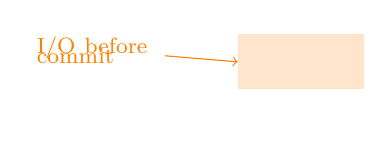
\begin{tikzpicture}every node/.style={inner sep=0,outer sep=0}]
\fill [orange!20] (0.8,0.3) rectangle (2.4,1);
\node (io) at (-1,0.8) [orange,text width=1.5cm] {\footnotesize I/O before\\[-1em]commit};
\draw[->,orange] (io) -- (0.8,0.65);
\node[anchor=south west,inner sep=0pt,outer sep=0pt] at (0,0) {\scalebox{0.75}{\usebox{\undoLoggingExample}}};
\end{tikzpicture}
\end{center}

\vskip1em

\begin{block}{Undo logging is \textbf{I/O intensive}}
\begin{itemize}[-]
\item Transactions only become ``permanent'' after they commit in the log;
\item but undo logging requires \textbf{writing the data before} committing in the log.
\end{itemize}
\end{block}

\end{frame}

%
%  ----------------------------------------
%
\begin{frame}{Buffer management with Undo Logging}


\begin{center}
\scalebox{0.9}{
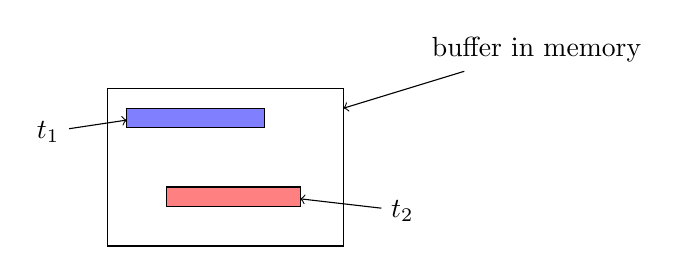
\begin{tikzpicture}every node/.style={inner sep=0,outer sep=0}]
\draw (0,0) rectangle (3,2);
\node (buffer) [anchor=west] at (4,2.5) {buffer in memory}; \draw [->] (buffer) -- (3,1.75);
\draw [fill=blue!50] (0.25,1.75) rectangle (2,1.5);
\draw [fill=red!50] (0.75,0.75) rectangle (2.45,0.5);

\node (t1) at (-0.75,1.45) {$t_1$}; \draw [->] (t1) -- (0.25,1.6);
\node (t2) at (3.75,0.45) {$t_2$}; \draw [->] (t2) -- (2.45,0.6);
\end{tikzpicture}}
\end{center}

Suppose transactions $T_1$, $T_2$ modify \textbf{different tuples} $t_1$ and $t_2$ in the \textbf{same block} (loaded to the same memory buffer), and that $T_1$ is ready to write its changes to disk and then commit.

Because \alert{I/O is performed one page at a time}, writing the changes of $T_1$ will also write \alert{\textbf{dirty}} data created by $T_2$. 

The DBMS \alert{must hold off on $T_1$'s commit until $T_2$ is ready to commit}. Otherwise, if $T_2$ aborts later on, the DBMS will have to bring the data back from disk to undo the change.

\end{frame}

%%%%%%%%%%%%% --- REDO LOGGING

%
% ----------------------------------------
%
\begin{frame}{Redo Logging}

\textbf{Idea}: save the results of the transaction to the log and commit the transaction as soon as the log has all new values. If there is a problem, \emph{replay} the log.

\textbf{Rules:}
\begin{enumerate}[label=(\arabic*)]
\item on a call to \WRITE{X}{v} by the transaction, write to the log the \textbf{new} value of database element \texttt{X}
\item only call \OUTPUT{X} after the transaction is committed on the log and the log has been \emph{flushed}
\end{enumerate}

\vskip1em

\begin{block}{Write Ahead Logging (WAL)}
Write all new values of the database elements to the log before writing them to disk.
\end{block}
\end{frame}

\newsavebox\redoLoggingExample
\savebox{\redoLoggingExample}{%
	\footnotesize
	\begin{tabular}{r|l|r|r|r|r|r|l}
& & & \multicolumn{2}{|c|}{Memory} & \multicolumn{2}{|c|}{Disk} & \\
\cline{4-7}
\raisebox{0.75em}{Step} & \raisebox{0.75em}{Action} & \raisebox{0.75em}{\texttt{v}} & \texttt{A} & \texttt{B} & \texttt{A} &\texttt{B} & \raisebox{0.75em}{Log} \\
\hline
1 & &&&& 75 & 40 & \LOGSTART{1}\\
2 & \READ{A}{v} & 75 & 75 &  & 75 & 40 \\
3 & \ASSIGN{v}{v-20} & 55 & 75 &  & 75 & 40 \\
4 & \WRITE{A}{v} & 55 & 55 &  & 75 & 40 & \LOGREDO{1}{A}{55}\\
5 & \READ{B}{v} & 40 & 55 & 40 & 75 & 40 \\
6 & \ASSIGN{v}{v+20} & 60 & 55 & 40 & 75 & 40 \\
7 & \WRITE{B}{v} & 60 & 55 & 60 & 75 & 40 & \LOGREDO{1}{B}{60}\\
8 & \COMMIT  & & 55 & 60 & 75 & 40 &  \LOGCOMMIT{1} \\
9 & \OUTPUT{A} & & 55 & 60 & 55 & 40  \\
10 & \OUTPUT{B} & & 55 & 60 & 55 & 60 
\end{tabular}
}

%
% ----------------------------------------
%
\begin{frame}

Redo Logging Example

\vskip1.5em

\begin{tikzpicture}
\node[anchor=south west,inner sep=0pt,outer sep=0pt] at (0,0) {\scalebox{0.9}{\usebox{\redoLoggingExample}}};
\pause
\node (1) at (10,1.975) [color=red,text width=3cm] {\footnotesize log has new values};
\node (2) at (7.975, 2.625) [draw, circle, minimum size=1.1em,color=red] { };
\node (3) at (7.975, 1.4) [draw, circle, minimum size=1.1em,color=red] { };
\draw [->,red] (1) -- (2) ;
\draw [->,red] (1) -- (3) ;
\pause
\node (4) at (4,-1) [color=blue,text width=3cm] {\footnotesize table has new values};
\node (5) at (5.375, 0.6) [draw, circle, minimum size=1.1em,color=blue] { };
\node (6) at (6.05, 0.2) [draw, circle, minimum size=1.1em,color=blue] { };
\draw [->,blue] (4) -- (5) ;
\draw [->,blue] (4) -- (6) ;
\end{tikzpicture}

\end{frame}

%
% ----------------------------------------
%
\begin{frame}{Crash Recovery with Redo Logging}

\scalebox{0.75}{\begin{minipage}{1.35\textwidth}%
\begin{algorithm}[H]
\begin{algorithmic}[1]
\State Scan the log to find all transactions that started and all transactions that committed
\State Read the log from the beginning towards the end
\ForEach{log entry $\langle e_i\rangle$}
	\If{$\langle e_i\rangle$ = \LOGREDO{j}{X}{v} \textbf{and} $T_j$ has committed} \Comment{must redo $T_j$}
		\State write $v$ as the value of \texttt{X} on the database \label{redoLoggingWritingNewValue}
	\EndIf
\EndFor
\ForEach{uncommitted transaction $T_i$}
	\State \alert{write \LOGABORT{i}} in the log \Comment{so that we ignore this transaction in the future}
\EndFor
\State flush the log
\caption{database recovery from Redo Log after system crash}
\end{algorithmic}
\end{algorithm}
\end{minipage}}
\end{frame}

%
% ----------------------------------------
%
\begin{frame}{Atomicity with Redo Logging}
\label{redo_logging_correctness_proof}

Proving that the Redo Logging protocol ensures atomicity requires showing that, with or without a system crash, no database element \texttt{X} has a value $v$ written by a transaction $T_j$ that \textbf{did not commit}.\footnote{Completing the proof to show that all writes of committed transactions are made persistent is left as an exercise.}

\underline{Case 1}: there was no system crash
\begin{itemize}[-,topsep=-0.5em]
\item $T_j$ aborted because some of its logical operations failed, \textbf{before} any \OUTPUT{X} \textbf{could have been called}.
\end{itemize}

\underline{Case 2}: there was a system crash
\begin{itemize}[-,topsep=-0.5em]
\item Line \ref{redoLoggingWritingNewValue} of the crash recovery algorithm, which does the writing, does not apply to transaction $T_j$ because it did not commit in the log.
\end{itemize}

\vskip1em
\end{frame}

%
% ----------------------------------------
%
\begin{frame}[fragile]{Re-doing a transaction already done?}

Because (with REDO logging) transactions commit in the log \textbf{before} writing changes to disk, the DBMS can never know (based on the log alone) if the results of a transaction are on disk or not.

\vskip1em

\begin{columns}[onlytextwidth]
\begin{column}{0.2\textwidth}
Example:
\end{column}
\begin{column}{0.8\textwidth}
\begin{center}
\scalebox{0.9}{
\begin{tikzpicture}[semithick,every node/.append style={font=\footnotesize}]
\begin{scope}[>=latex]
\draw [->] (0,1) -- (8,1); \node (caption) at (8.5,1) {time};
\draw [|-|] (0.5,2.5) -- (2.5,2.5) node [midway,yshift=-5pt,label=above:{$T_1$}] {};
\draw [|-] (2,2) -- (4,2) node [midway,yshift=-5pt,label=above:{$T_2$}] {};
\end{scope}

\node (C1) at (2.5,0.5) [red] {\LOGCOMMIT{1}};
\draw[->,red] (C1) -- (2.5,1);

\draw[dashed] (4,0.8) -- (4,3.25); % crash
\draw[dashed] (5.5,0.8) -- (5.5,3.25); % recovery
\draw[dashed] (7.125,0.8) -- (7.125,3.25); % ready

\node [xshift=20pt,rotate=30,text width=1.75cm,red] at (4,0.85) {\footnotesize {crash}};
\node [xshift=20pt,rotate=30,text width=1.75cm] at (5.5,0.85) {\footnotesize {restart}};
\node [xshift=20pt,rotate=30,text width=1.75cm,blue] at (7.125,0.85) {\footnotesize {ready}};

\node (r0) at (6.35,3.5) [red] {recovery};
\node (r1) at (6.25,2.5) {redo $T_1$};
\node (r2) at (6.25,2) {abort $T_2$};

\end{tikzpicture}}
\end{center}
\end{column}
\end{columns}

The DBMS \textbf{must redo} $T_1$ (and every other committed transaction in the log) after a crash, \textbf{even if it had written its changes to disk}.

\vskip0.5em

\emph{\alert{Periodic checkpointing}}, discussed next, solves this problem.

\end{frame}

%
% ----------------------------------------
%
\begin{frame}[fragile]

\vskip2em

\textbf{Quiescent}\footnotemark checkpointing


\begin{center}
\scalebox{0.9}{
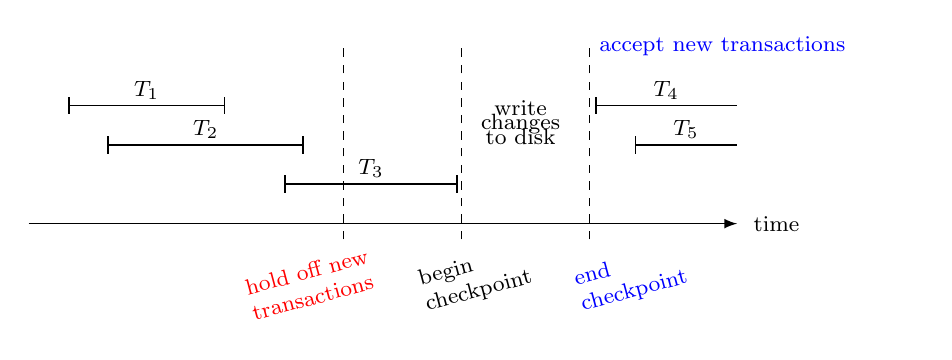
\begin{tikzpicture}[semithick,every node/.append style={font=\footnotesize}]
\begin{scope}[>=latex]
\draw [->] (0,1) -- (9,1); \node (caption) at (9.5,1) {time};
\draw [|-|] (0.5,2.5) -- (2.5,2.5) node [midway,yshift=-5pt,label=above:{$T_1$}] {};
\draw [|-|] (1,2) -- (3.5,2) node [midway,yshift=-5pt,label=above:{$T_2$}] {};
\draw [|-|] (3.25,1.5) -- (5.45,1.5) node [midway,yshift=-5pt,label=above:{$T_3$}] {};
\end{scope}

\draw[dashed] (4,0.8) -- (4,3.25); % hold new transactions
\draw[dashed] (5.5,0.8) -- (5.5,3.25); % begin chptk
\draw[dashed] (7.125,0.8) -- (7.125,3.25); % end chkpt

\node [xshift=-10pt,rotate=15,text width=1.75cm,red] at (4,0.25) {\footnotesize {hold off new transactions}};
\node [xshift=10pt,rotate=15,text width=1.75cm] at (5.5,0.35) {\footnotesize {begin\\checkpoint}};
\node [xshift=20pt,rotate=15,text width=1.75cm,blue] at (7.125,0.35) {\footnotesize {end\\checkpoint}};

\node (c1) at (6.25,2.5) [text width=2cm] {\begin{center}\footnotesize \alert{write\\[-0.5em]changes\\[-0.5em]to disk}\end{center}};

\draw [|-] (7.2,2.5) -- (9,2.5) node [midway,yshift=-5pt,label=above:{$T_4$}] {};
\draw [|-] (7.7,2) -- (9,2) node [midway,yshift=-5pt,label=above:{$T_5$}] {};

\node (c1) at (9.25,3.25) [text width=4cm,blue] {\footnotesize accept new transactions };

\end{tikzpicture}}
\end{center}

When the DBMS decides to do a checkpoint, it: (1) \textbf{stops} accepting transactions; (2) writes to disk all changes by previous transactions; and then (3) resumes.

\vskip2em

\footnotetext{To \textbf{quiesce} is to \alert{pause} or alter a device or application \alert{to achieve a consistent state}, usually in preparation for a backup or other maintenance.\\ \url{https://en.wikipedia.org/wiki/Quiesce}}
\end{frame}

\newsavebox\nonquiescentCheckpointing
\savebox{\nonquiescentCheckpointing}{
\footnotesize
\begin{tabular}{r@{~}l}
&$\vdots$\\
&\LOGSTART{y} \\
&\LOGUNDO{x}{A}{7}\\
&\LOGUNDO{y}{C}{19}\\
\textcolor{red}{$\rightarrow$}&\LOGBEGINCKPT{$T_x, T_y$} \\
&\LOGSTART{z} \\
&\LOGUNDO{z}{D}{23}\\
&\LOGCOMMIT{x}\\
&\LOGSTART{w}\\
&\LOGABORT{y}\\
\textcolor{red}{$\rightarrow$}&\LOGENDCKPT\\
&\LOGUNDO{w}{E}{29}\\
&\LOGCOMMIT{z}\\
&\LOGUNDO{w}{E}{29}\\
&\LOGUNDO{w}{F}{31}\\
&$\vdots$\\
\end{tabular}}

%
% ----------------------------------------
%
\begin{frame}[fragile]
\label{nonquiescent_checkpointing}

A \textbf{Nonquiescent} checkpoint applies only to transactions that \textbf{committed before the checkpoint started}.

\begin{center}
\scalebox{0.9}{
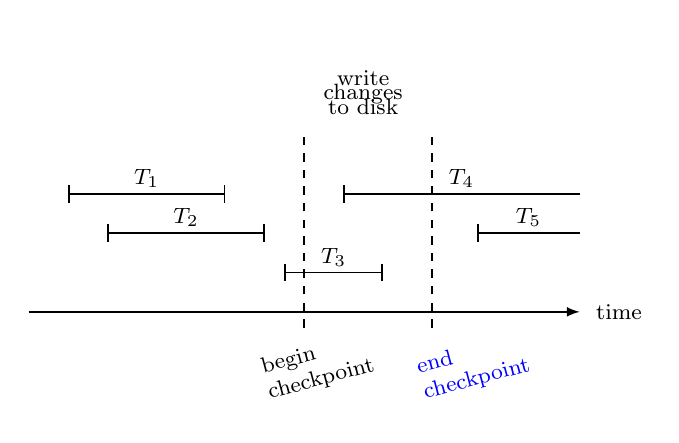
\begin{tikzpicture}[semithick,every node/.append style={font=\footnotesize}]
\begin{scope}[>=latex]
\draw [->] (2,1) -- (9,1); \node (caption) at (9.5,1) {time};
\draw [|-|] (2.5,2.5) -- (4.5,2.5) node [midway,yshift=-5pt,label=above:{$T_1$}] {};
\draw [|-|] (3,2) -- (5,2) node [midway,yshift=-5pt,label=above:{$T_2$}] {};
\draw [|-|] (5.25,1.5) -- (6.5,1.5) node [midway,yshift=-5pt,label=above:{$T_3$}] {};
\end{scope}

\draw[dashed] (5.5,0.8) -- (5.5,3.25); % begin chptk
\draw[dashed] (7.125,0.8) -- (7.125,3.25); % end chkpt

\node [xshift=10pt,rotate=15,text width=1.75cm] at (5.5,0.35) {\footnotesize {begin\\checkpoint}};
\node [xshift=20pt,rotate=15,text width=1.75cm,blue] at (7.125,0.35) {\footnotesize {end\\checkpoint}};

\node (c1) at (6.25,4) [text width=2cm] {\begin{center}\footnotesize \alert{write\\[-0.5em]changes\\[-0.5em]to disk}\end{center}};

\draw [|-] (6,2.5) -- (9,2.5) node [midway,yshift=-5pt,label=above:{$T_4$}] {};
\draw [|-] (7.7,2) -- (9,2) node [midway,yshift=-5pt,label=above:{$T_5$}] {};
\end{tikzpicture}}
\end{center}

In the example above, changes by $T_1$ and $T_2$ are forced to disk, and they become ``100\%'' permanent.

All other transactions that commit will be re-done if there is a crash before the next checkpoint.

\end{frame}


\newsavebox{\sharedBuffersCheckpoint}
\savebox{\sharedBuffersCheckpoint}{
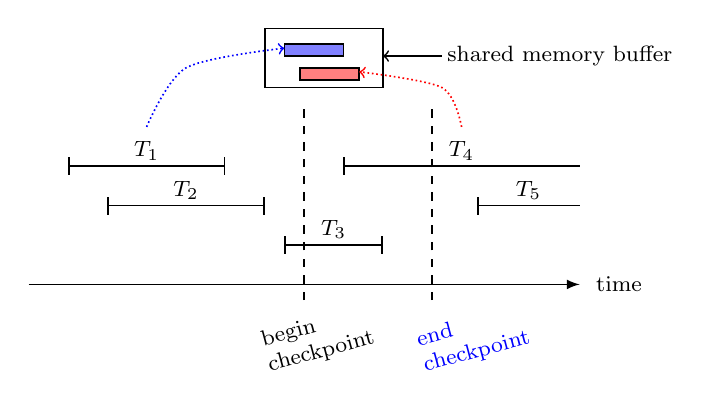
\begin{tikzpicture}[semithick,every node/.append style={font=\footnotesize}]
\begin{scope}[>=latex]
\draw [->] (2,1) -- (9,1); \node (caption) at (9.5,1) {time};
\draw [|-|] (2.5,2.5) -- (4.5,2.5) node [midway,yshift=-5pt,label=above:{$T_1$}] {};
\draw [|-|] (3,2) -- (5,2) node [midway,yshift=-5pt,label=above:{$T_2$}] {};
\draw [|-|] (5.25,1.5) -- (6.5,1.5) node [midway,yshift=-5pt,label=above:{$T_3$}] {};
\end{scope}

\draw[dashed] (5.5,0.8) -- (5.5,3.25); % begin chptk
\draw[dashed] (7.125,0.8) -- (7.125,3.25); % end chkpt

\node [xshift=10pt,rotate=15,text width=1.75cm] at (5.5,0.35) {begin\\checkpoint};
\node [xshift=20pt,rotate=15,text width=1.75cm,blue] at (7.125,0.35) {end\\checkpoint};

\draw [|-] (6,2.5) -- (9,2.5) node [midway,yshift=-5pt,label=above:{$T_4$}] {};
\draw [|-] (7.7,2) -- (9,2) node [midway,yshift=-5pt,label=above:{$T_5$}] {};

%
% shared buffer
%
\draw (5,3.5) rectangle (6.5,4.25); 
\node (buffer) [anchor=west,inner sep=0pt,outer sep=2pt] at (7.25,3.9) {shared memory buffer};
\draw[->] (buffer) -- (6.5,3.9);

\draw [fill=blue!50] (5.25,3.9) rectangle (6,4.05); %tuple used by T1
\draw [fill=red!50] (5.45,3.6) rectangle (6.2,3.75); %tuple used by T4

\draw[->,densely dotted,blue] plot [smooth] coordinates {(3.5,3) (4,3.75) (5.25,4)};
\draw[->,densely dotted,red] plot [smooth] coordinates {(7.5,3) (7.25,3.5) (6.2,3.7)};

\end{tikzpicture}
}
%
% ----------------------------------------
%
\begin{frame}{Buffer management with Redo Logging}

What if a committed transaction shares a buffer with an uncommitted transaction excluded from the checkpoint?

\vskip1em

\begin{center}
\scalebox{0.9}{\usebox{\sharedBuffersCheckpoint}}
\end{center}

The checkpoint cannot proceed until $T_4$ commits! Alternatively, the DBMS may \alert{hold off \textbf{starting} $T_4$ (only) until the checkpoint is complete}.


\end{frame}

%
% ----------------------------------------
%
\begin{frame}{Summary}

The logging strategies we've seen so far...

\begin{itemize}[-,noitemsep]
\item Undo logging is \textbf{I/O intensive}: write changes before committing.
\item Redo logging is \textbf{memory intensive}: write changes after committing. 
\end{itemize}

In both cases, sharing buffers can be difficult, forcing the DBMS to hold off the execution of some transactions.

\vskip1em

Long-running transactions are especially problematic: they need a lot of memory with Redo logging, and may hold off other transactions for a long time.
\end{frame}

%
% ----------------------------------------
%
\begin{frame}{Undo/Redo Logging}
Arriving at the best of both worlds...

\textbf{Rules}:
\begin{enumerate}[label=(\arabic*)]
\item on \WRITE{X}{v}, write \textbf{both} the old and the new values of \texttt{X} on the log
\item flush the log immediately after the transaction commits
\item flush dirty buffers anytime
\end{enumerate}

\vskip1em

\begin{block}{Write Ahead Logging (WAL)}
For every database element, the log \alert{must have} its old and new values \textbf{before} the dirty buffer with that element is flushed.
\end{block}
\end{frame}

\newsavebox\undoRedoLoggingExample
\savebox{\undoRedoLoggingExample}{%
	\footnotesize
\begin{tabular}{r|l|r|r|r|r|r|l}
& & & \multicolumn{2}{|c|}{Memory} & \multicolumn{2}{|c|}{Disk} & \\
\cline{4-7}
\raisebox{0.5em}{Step} & \raisebox{0.5em}{Action} & \raisebox{0.5em}{\texttt{v}} & \texttt{A} & \texttt{B} & \texttt{A} & \texttt{B} & \raisebox{0.5em}{Log} \\
\hline
1 & &&&& 75 & 40 & \LOGSTART{1}\\
2 & \READ{A}{v} & 75 & 75 &  & 75 & 40 \\
3 & \ASSIGN{v}{v-20} & 55 & 75 &  & 75 & 40 \\
4 & \WRITE{A}{v} & 55 & 55 &  & 75 & 40 & \LOGUNDOREDO{1}{A}{75}{55}\\
5 & \READ{B}{v} & 40 & 55 & 40 & 75 & 40 \\
6 & \ASSIGN{v}{v+20} & 60 & 55 & 40 & 75 & 40 \\
7 & \WRITE{B}{v} & 60 & 55 & 60 & 75 & 40 & \LOGUNDOREDO{1}{B}{40}{60}\\
10 & \OUTPUT{B} &  & 55 & 60 & 55 & 60  \\
9 & \COMMIT &  & 55 & 60 & 55 & 60 &  \LOGCOMMIT{1} \\
10 & \OUTPUT{A} &  & 75 & 40 & 55 & 60 
\end{tabular}
}

%
% ----------------------------------------
%
\begin{frame}
Undo/Redo Logging Example

\vskip1.5em

\begin{tikzpicture}
\node[anchor=south west,inner sep=0pt,outer sep=0pt] at (0,0) {\scalebox{0.9}{\usebox{\undoRedoLoggingExample}}};
\pause
\node (1) at (11,4) [color=red,text width=3cm] {\footnotesize log has\\[-0.5em]old values};
\node (2) at (8, 2.6) [draw, circle, minimum size=1.1em,color=red] { };
\node (3) at (8, 1.4) [draw, circle, minimum size=1.1em,color=red] { };
\draw [->,red] ([xshift=10pt,yshift=3pt]1.south west) -- (2) ;
\draw [-,red] (2) -- (3) ;
\pause
\node (4) at (11,2.5) [color=blue,text width=3cm] {\footnotesize log has\\[-0.5em]new values};
\node (5) at (8.525, 2.6) [draw, circle, minimum size=1.1em,color=blue] { };
\node (6) at (8.525, 1.4) [draw, circle, minimum size=1.1em,color=blue] { };
\draw [->,blue] (4) -- (6) ;
\draw [-,blue] (5) -- (6) ;
\pause
\node (7) at (9,0.25) [color=blue,text width=3cm] {\footnotesize table has new values};
\node (8) at (5.375, 1) [draw, circle, minimum size=1.1em,color=blue] { };
\node (9) at (6.05, 0.2) [draw, circle, minimum size=1.1em,color=blue] { };
\draw [->,blue] (7.mid west) -- (6,0.8) -- (8) ;
\draw [->,blue] (7) -- (9) ;
\end{tikzpicture}
\end{frame}

%
% ----------------------------------------
%
\begin{frame}

\textbf{Crash Recovery} with Undo/Redo Logging:

\begin{enumerate}[(1),noitemsep]
\item read the log backwards until a checkpoint; 
\item find out which transactions completed, and which didn't;
\item \textbf{undo} all transactions that did not complete; mark them as aborted in the log;
\item \textbf{redo} all transactions that committed but started since the most recent \emph{checkpoint}.
\end{enumerate}

\vskip1em

\textbf{Atomicity} with Undo/Redo Logging:

A similar argument to the previous protocols works.

\end{frame}

%
% ----------------------------------------
%

\begin{frame}{Checkpointing with Undo/Redo logging}

\begin{center}
\scalebox{0.75}{\usebox{\sharedBuffersCheckpoint}}
\end{center}

With Undo/Redo logging we are free to write to disk anytime we want, regardless of the state of the transaction.

We can flush the shared buffer with the uncommited changes of $T_2$ during the checkpoint of $T_1$, because if $T_2$ aborts we have the old value in the log to perform the undo.

\end{frame}


%
% ----------------------------------------
%
\begin{frame}{What else about logging?}

\begin{BOX}{Backups}
The log can be used to enable \underline{incremental backups} of the database that work pretty much like checkpointing, except that instead of flushing dirty buffers to disk, the system \emph{replays} the log on the backup database.
\end{BOX}

\vskip1em

\begin{BOX}{Reusing the log}
The log file can be truncated periodically, once all transactions are safely preserved (e.g., after backups or checkpoints). 

\vskip0.5em

Some systems use a fixed-sized circular buffer for the log.
\end{BOX}

\end{frame}

%
% ----------------------------------------
%
\begin{frame}{Replication with Undo/Redo Logging}

Redo Logs can be used to keep a replica database up-to-date:\\
 - the master sends the log entries while the replica periodically acknowledges which transactions have been replicated\\
 - the replica can take over on a failure of the master system

\vskip1em
 
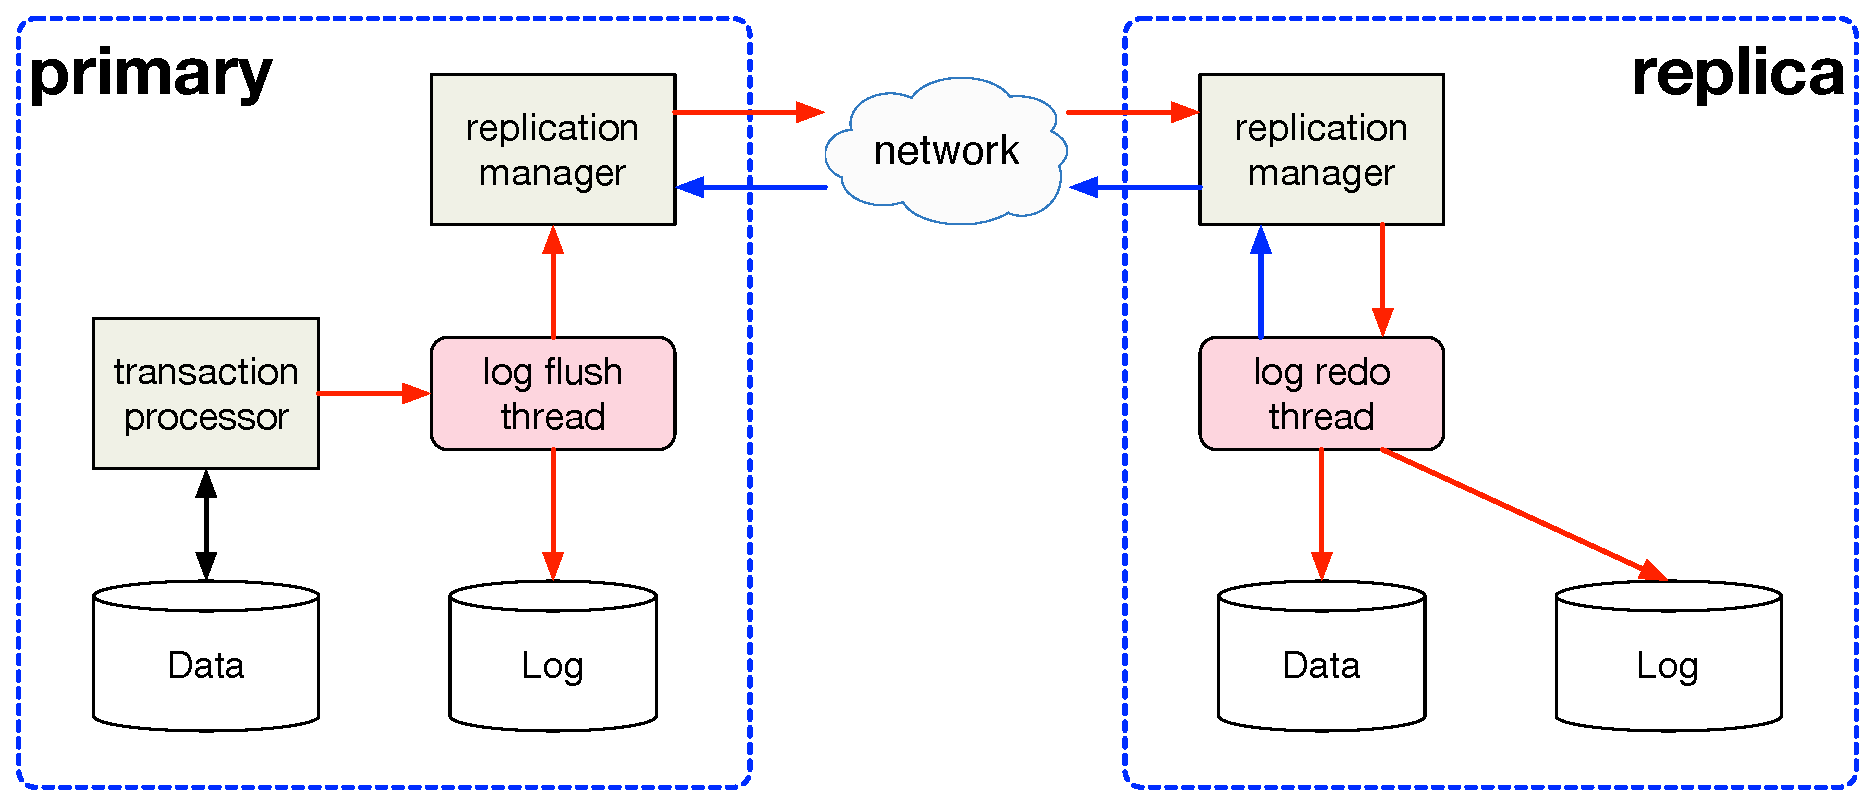
\includegraphics[width=\textwidth]{figures/redo_logging_replication}
\end{frame}



%
% ----------------------------------------
%
\begin{frame}{Logging and Durability}

Two sides to the story:
\begin{enumerate}[(1),noitemsep,topsep=-0.5em]
 \item Recovering from a crash (logging).
 \item Preventing/recovering from media failure.
\end{enumerate}
\vskip2em

Media \textbf{reliability} can be improved by:
\begin{enumerate}[(1),noitemsep,topsep=-0.5em]
 \item Buying better hardware.
 \item Adding \textbf{redundancy}.
\end{enumerate}
\vskip1em

Many forms of redundancy:
\begin{enumerate}[(1),noitemsep,topsep=-0.5em]
 \item RAID: having the same data written to multiple disks.
 \item Replication: having a DBMS act as a hot backup of another.
\end{enumerate}


\end{frame}
